\documentclass[12pt]{article}
\usepackage[utf8]{inputenc}
\usepackage[russian]{babel}
\usepackage{amsmath}
\usepackage{amssymb}
\usepackage{geometry}
\usepackage{graphicx}
\geometry{a4paper, margin=1in}
\usepackage{listings}
\usepackage{xcolor}

\lstset{
  language=C++,                % Язык программирования
  basicstyle=\ttfamily\small,  % Шрифт и размер текста
  keywordstyle=\color{blue},   % Цвет ключевых слов
  commentstyle=\color{gray},   % Цвет комментариев
  stringstyle=\color{red},     % Цвет строк
  numbers=left,                % Нумерация строк слева
  numberstyle=\tiny\color{gray}, % Стиль номеров строк
  stepnumber=1,                % Интервал нумерации строк
  breaklines=true,             % Перенос длинных строк
  frame=single,                % Рамка вокруг кода
}

\title{Отчёт по расчётной работе по дисциплине ПиОИвИС}
\author{}
\date{}


\begin{document}

\maketitle

\begin{center}
\section*{Графы}
\end{center}

\subsection*{Цель}
Найти объединение множества неориентированных графов

\subsection*{Вариант}
4.8 мc

\section*{Определения}

\begin{itemize}
    \item \textbf{Граф} —  математическая абстракция реальной системы любой природы, объекты которой обладают парными связями. Граф как математический объект есть совокупность двух множеств — множества самих объектов, называемого множеством вершин, и множества их парных связей, называемого множеством рёбер. Элемент множества рёбер есть пара элементов множества вершин.
    
    
    \item \textbf{Неориентрованный граф} — это граф у которого рёбра не указывают направление. Это значит, что из любой вершины можно попасть в любую точку графа.
    
    
     
\includegraphics[width=0.7\textwidth, height=5cm, keepaspectratio]{1.png}
     
    \item \textbf{Сме́жность} — непосредственная близость, примыкание. В теории графов смежность вершин соответствует наличию ребра между ними.
    
    \item \textbf{Матрица смежности} - это вид представления графа в виде матрицы, когда пересечение столбцов и строк задаёт дуги.
    
        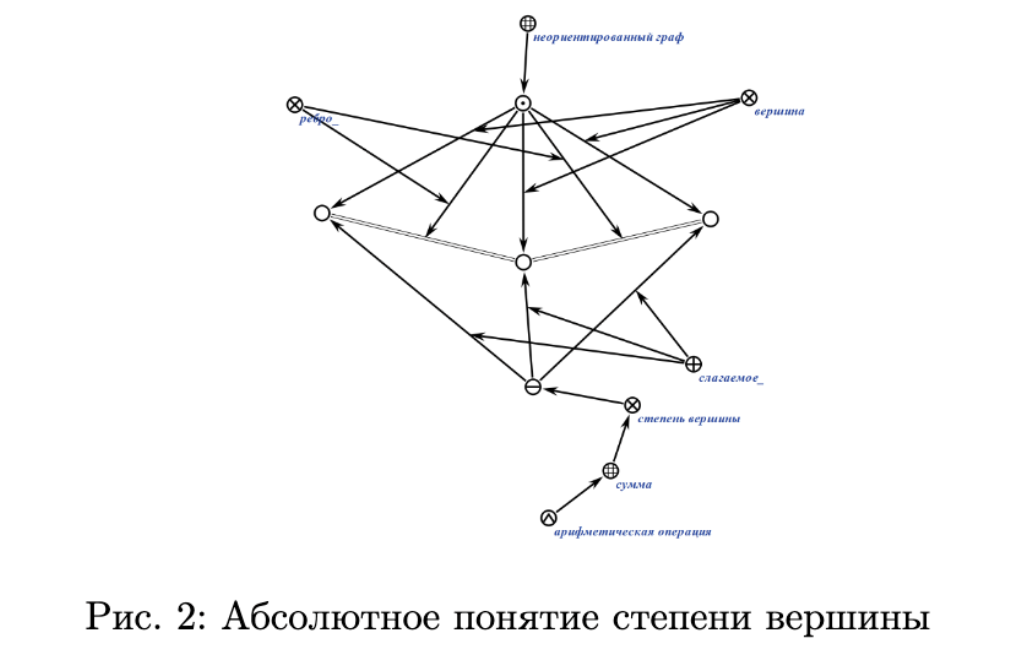
\includegraphics[width=0.8\textwidth, height=10cm, keepaspectratio]{2.jpeg}
        
\end{itemize}

\section*{Алгоритм}
\begin{enumerate}
    \item Создаётся пустой граф unionGraph для объединения графов.
    \item Ввод первого графа.
    \item Ввод второго графа.
    \item Подгон размера матриц с помощью resizeMatrix.
    \item Объединение графов функцией UnionGraphs() .
    \item Считать первый и второй граф из файла graph1.txt и graph2.txt с помощью readGraphFromFile() и объединить его с unionGraph.
    \item Используя displayGraph() вывести итоговую матрицу смежности объединенного графа.
    
\end{enumerate}
\section*{Код}
\begin{lstlisting}
#include <iostream> 
#include <vector> 
#include <fstream> 
using namespace std;

class Graph {
private:
    vector<vector<int>> Matrix_smezh;
public:
    Graph(int razmer = 0) {
        Matrix_smezh.resize(razmer, vector<int>(razmer, 0));
    }

    void addRebro(int v1, int v2, int ves) {
        if (v1 < Matrix_smezh.size() && v2 < Matrix_smezh.size()) {
            Matrix_smezh[v1][v2] = ves;
            Matrix_smezh[v2][v1] = ves; // Для неориентированного графа 
        }
    }

    void UnionGraphs(const Graph& drugoy) {
        int maxSize = max(Matrix_smezh.size(), drugoy.Matrix_smezh.size());
        resizeMatrix(maxSize);
        for (int i = 0; i < drugoy.Matrix_smezh.size(); ++i) {
            for (int j = 0; j < drugoy.Matrix_smezh[i].size(); ++j) {
                if (drugoy.Matrix_smezh[i][j]) {
                    Matrix_smezh[i][j] = drugoy.Matrix_smezh[i][j];
                }
            }
        }
    }

    void displayGraph() const {
        cout << "Matrica Smejnosti:" << endl;
        for (const auto& row : Matrix_smezh) {
            for (int val : row) {
                cout << val << " ";
            }
            cout << endl;
        }
    }

    void resizeMatrix(int newSize) {
        Matrix_smezh.resize(newSize);
        for (auto& row : Matrix_smezh) {
            row.resize(newSize, 0);
        }
    }

    const vector<vector<int>>& getMatrix_smezh() const {
        return Matrix_smezh;
    }
};

void writeGraphToFile(const Graph& graph, const string& filename) {
    ofstream file(filename);
    if (!file.is_open()) {
        cout << "Ne ydalos otkrit file: " << filename << endl;
        return;
    }
    const auto& Matrix_smezh = graph.getMatrix_smezh();
    file << Matrix_smezh.size() << endl;
    for (const auto& row : Matrix_smezh) {
        for (int val : row) {
            file << val << " ";
        }
        file << endl;
    }
    file.close();
    cout << "Graph zapisan v file " << filename << endl;
}

void readGraphFromFile(Graph& graph, const string& filename) {
    ifstream file(filename);
    if (!file.is_open()) {
        cout << "Ne ydalos otkrit file: " << filename << endl;
        return;
    }
    int size;
    file >> size;
    Graph tempGraph(size);
    for (int i = 0; i < size; ++i) {
        for (int j = 0; j < size; ++j) {
            int edge;
            file >> edge;
            tempGraph.addRebro(i, j, edge);
        }
    }
    graph.UnionGraphs(tempGraph);
    file.close();
}

Graph inputGraph() {
    int size;
    cout << "Vvedite razmer matrici smejnosti: ";
    cin >> size;
    Graph graph(size);
    cout << "Vvedite matricy smejnosty (po " << size << " chisel v kajdoi stroke):" << endl;
    for (int i = 0; i < size; ++i) {
        for (int j = 0; j < size; ++j) {
            int rebro;
            cin >> rebro;
            graph.addRebro(i, j, rebro);
        }
    }
    return graph;
}

int main() {
    Graph unionGraph;
    char vybor;
    setlocale(0, "");
    cout << "Vvesti novie graphs (y/n): ";
    cin >> vybor;
    if (vybor == 'y' || vybor == 'Y') {
        
        cout << "Vvedite dannie dlya pervogo grapha." << endl;
        Graph g1 = inputGraph();
        cout << "Save graph 1 in file (y/n): ";
        cin >> vybor;
        if (vybor == 'y' || vybor == 'Y') {
            string filename;
            cout << "Vvedite imya file : ";
            cin >> filename;
            if (filename.substr(filename.size() - 4) != ".txt") {
                filename += ".txt";
            }
            writeGraphToFile(g1, filename);
        }
       
        cout << "Vvedite dannie dlya pervogo grapha." << endl;
        Graph g2 = inputGraph();
        cout << "Save graph 2 in file (y/n): ";
        cin >> vybor;
        if (vybor == 'y' || vybor == 'Y') {
            string filename;
            cout << "Vvedite imya file dlya file 2 : ";
            cin >> filename;
            if (filename.substr(filename.size() - 4) != ".txt") {
                filename += ".txt";
            }
            writeGraphToFile(g2, filename);
        }
        
        unionGraph.UnionGraphs(g1);
        unionGraph.UnionGraphs(g2);
    }
    else {
       
        readGraphFromFile(unionGraph, "graph1.txt");
        readGraphFromFile(unionGraph, "graph2.txt");
    }
    cout << "Result:" << endl;
    unionGraph.displayGraph();
    return 0;
}


\end{lstlisting}
\section*{Пример работы кода}
 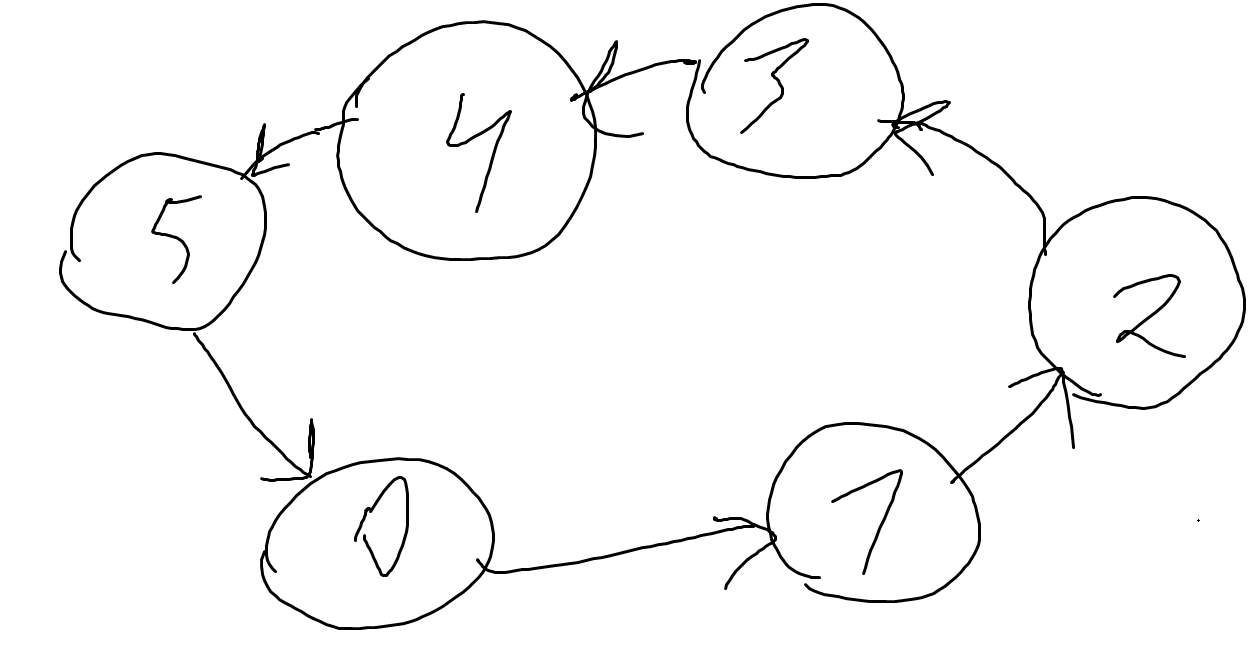
\includegraphics[width=0.9\textwidth, height=12cm, keepaspectratio]{3.jpg}
\section*{Вывод}

В результате выполнения данной работы были получены следующие практические навыки:

\begin{itemize}
    \item Изучены основы теории графов.
    \item Изучены способы представления графов.
    \item Изучены базовые алгоритмы для работы с графами.
\end{itemize}

\end{document}